
\subsection*{1.}

On a :

\(p(M) = \dfrac{30}{150} = \dfrac{1}{5} = 0{,}2\)

\(p(S) = \dfrac{45}{150} = \dfrac{3}{10} = 0{,}3\)

\(p(C) = 1 - (0{,}2 + 0{,}3) = 1 - 0{,}5 = 0{,}5\)

\begin{center}
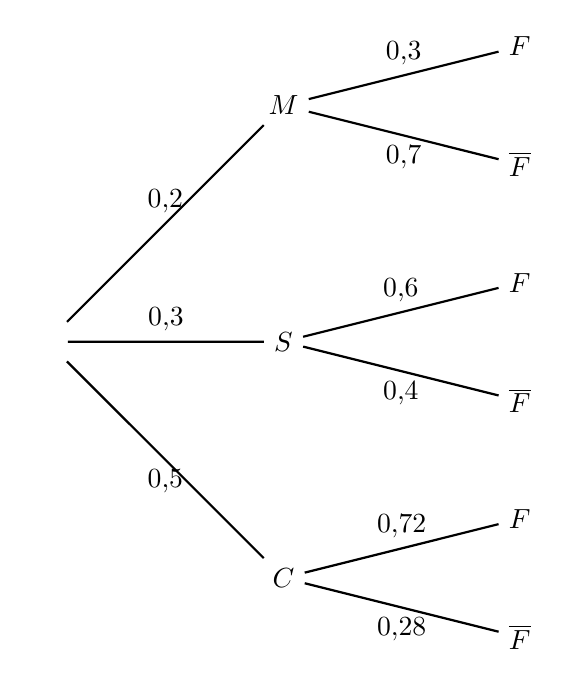
\begin{tikzpicture}[thick, scale=1.5]
\node (P_-1_0) at (-2,-2.5) {$\phantom{A}$};
\node (P_0_0) at (0,-0.5) {$M$};
\draw (P_-1_0) -- (P_0_0) node[midway, above] {$0{,}2$};
\node (P_1_0) at (2,-0) {$F$};
\draw (P_0_0) -- (P_1_0) node[midway, above] {$0{,}3$};
\node (P_1_1) at (2,-1) {$\overline{F}$};
\draw (P_0_0) -- (P_1_1) node[midway, below] {$0{,}7$};
\node (P_0_2) at (0,-2.5) {$S$};
\draw (P_-1_0) -- (P_0_2) node[midway, above] {$0{,}3$};
\node (P_1_2) at (2,-2) {$F$};
\draw (P_0_2) -- (P_1_2) node[midway, above] {$0{,}6$};
\node (P_1_3) at (2,-3) {$\overline{F}$};
\draw (P_0_2) -- (P_1_3) node[midway, below] {$0{,}4$};
\node (P_0_4) at (0,-4.5) {$C$};
\draw (P_-1_0) -- (P_0_4) node[midway, below] {$0{,}5$};
\node (P_1_4) at (2,-4) {$F$};
\draw (P_0_4) -- (P_1_4) node[midway, above] {$0{,}72$};
\node (P_1_5) at (2,-5) {$\overline{F}$};
\draw (P_0_4) -- (P_1_5) node[midway, below] {$0{,}28$};
\end{tikzpicture}
\end{center}

\subsection*{2.}

On calcule :
\[
p(F \cap M) = p(M \cap F) = p(M) \times p_M(F) = 0{,}2 \times 0{,}3 = 0{,}06.
\]

\subsection*{3.}

On a de même :
\[
p(F \cap S) = p(S \cap F) = p(S) \times p_S(F) = 0{,}3 \times 0{,}6 = 0{,}18,
\]
\[
p(F \cap C) = p(C \cap F) = p(C) \times p_C(F) = 0{,}5 \times 0{,}72 = 0{,}36.
\]
D'après la loi des probabilités totales :
\begin{align*}
p(F) &= p(F \cap M) + p(F \cap S) + p(F \cap C) \\
&= 0{,}06 + 0{,}18 + 0{,}36 \\
&= 0{,}60.
\end{align*}

\subsection*{4.}

On a :
\[
p(F \cap M) = 0{,}06 \quad \text{et} \quad p(F) \times p(M) = 0{,}6 \times 0{,}2 = 0{,}12,
\]
donc :
\[
p(F \cap M) \neq p(F) \times p(M),
\]
les évènements \(F\) et \(M\) ne sont pas indépendants.

\subsection*{5.}

On a \( p(F) = 0{,}6 \), donc \( p(\overline{F}) = 1 - 0{,}6 = 0{,}4 \) (probabilité de choisir un garçon).

Donc :
\[
p_{\overline{F}}(C) = \dfrac{p(\overline{F} \cap C)}{p(\overline{F})} = \dfrac{0{,}5 \times 0{,}28}{0{,}4} = \dfrac{0{,}14}{0{,}4} = \dfrac{14}{40} = 0{,}35.
\]

